\chapter{Bedienungsanleitung}\label{chap:bedienungsanleitung}


\section{Bedienen}

Im Normalfall liegt der Visual-Megesort als Datei mit der Endung \texttt{.jar} vor. Die Dateiendung JAR kennzeichnet Archive, die mehrere Java-Dateien und deren Metainformationen enthalten. Um die Datei ausführen zu können, muss die \texttt{Java Runtime Environment} installiert sein. Die Laufzeitumgebung kann gegebenenfalls kostenlos im Internet heruntergeladen werden.

Die Anwendung kann man durch einen Doppelklick, oder aus der Konsole durch den folgenden Aufruf starten.

\begin{verbatim}
java -jar Visual-Mergesort.jar
\end{verbatim}

Startet man die Applikation, so öffnet sich folgendes Fenster (Abbildung \ref{figure:start-app}):

\begin{figure}[!htb]
    \centering
      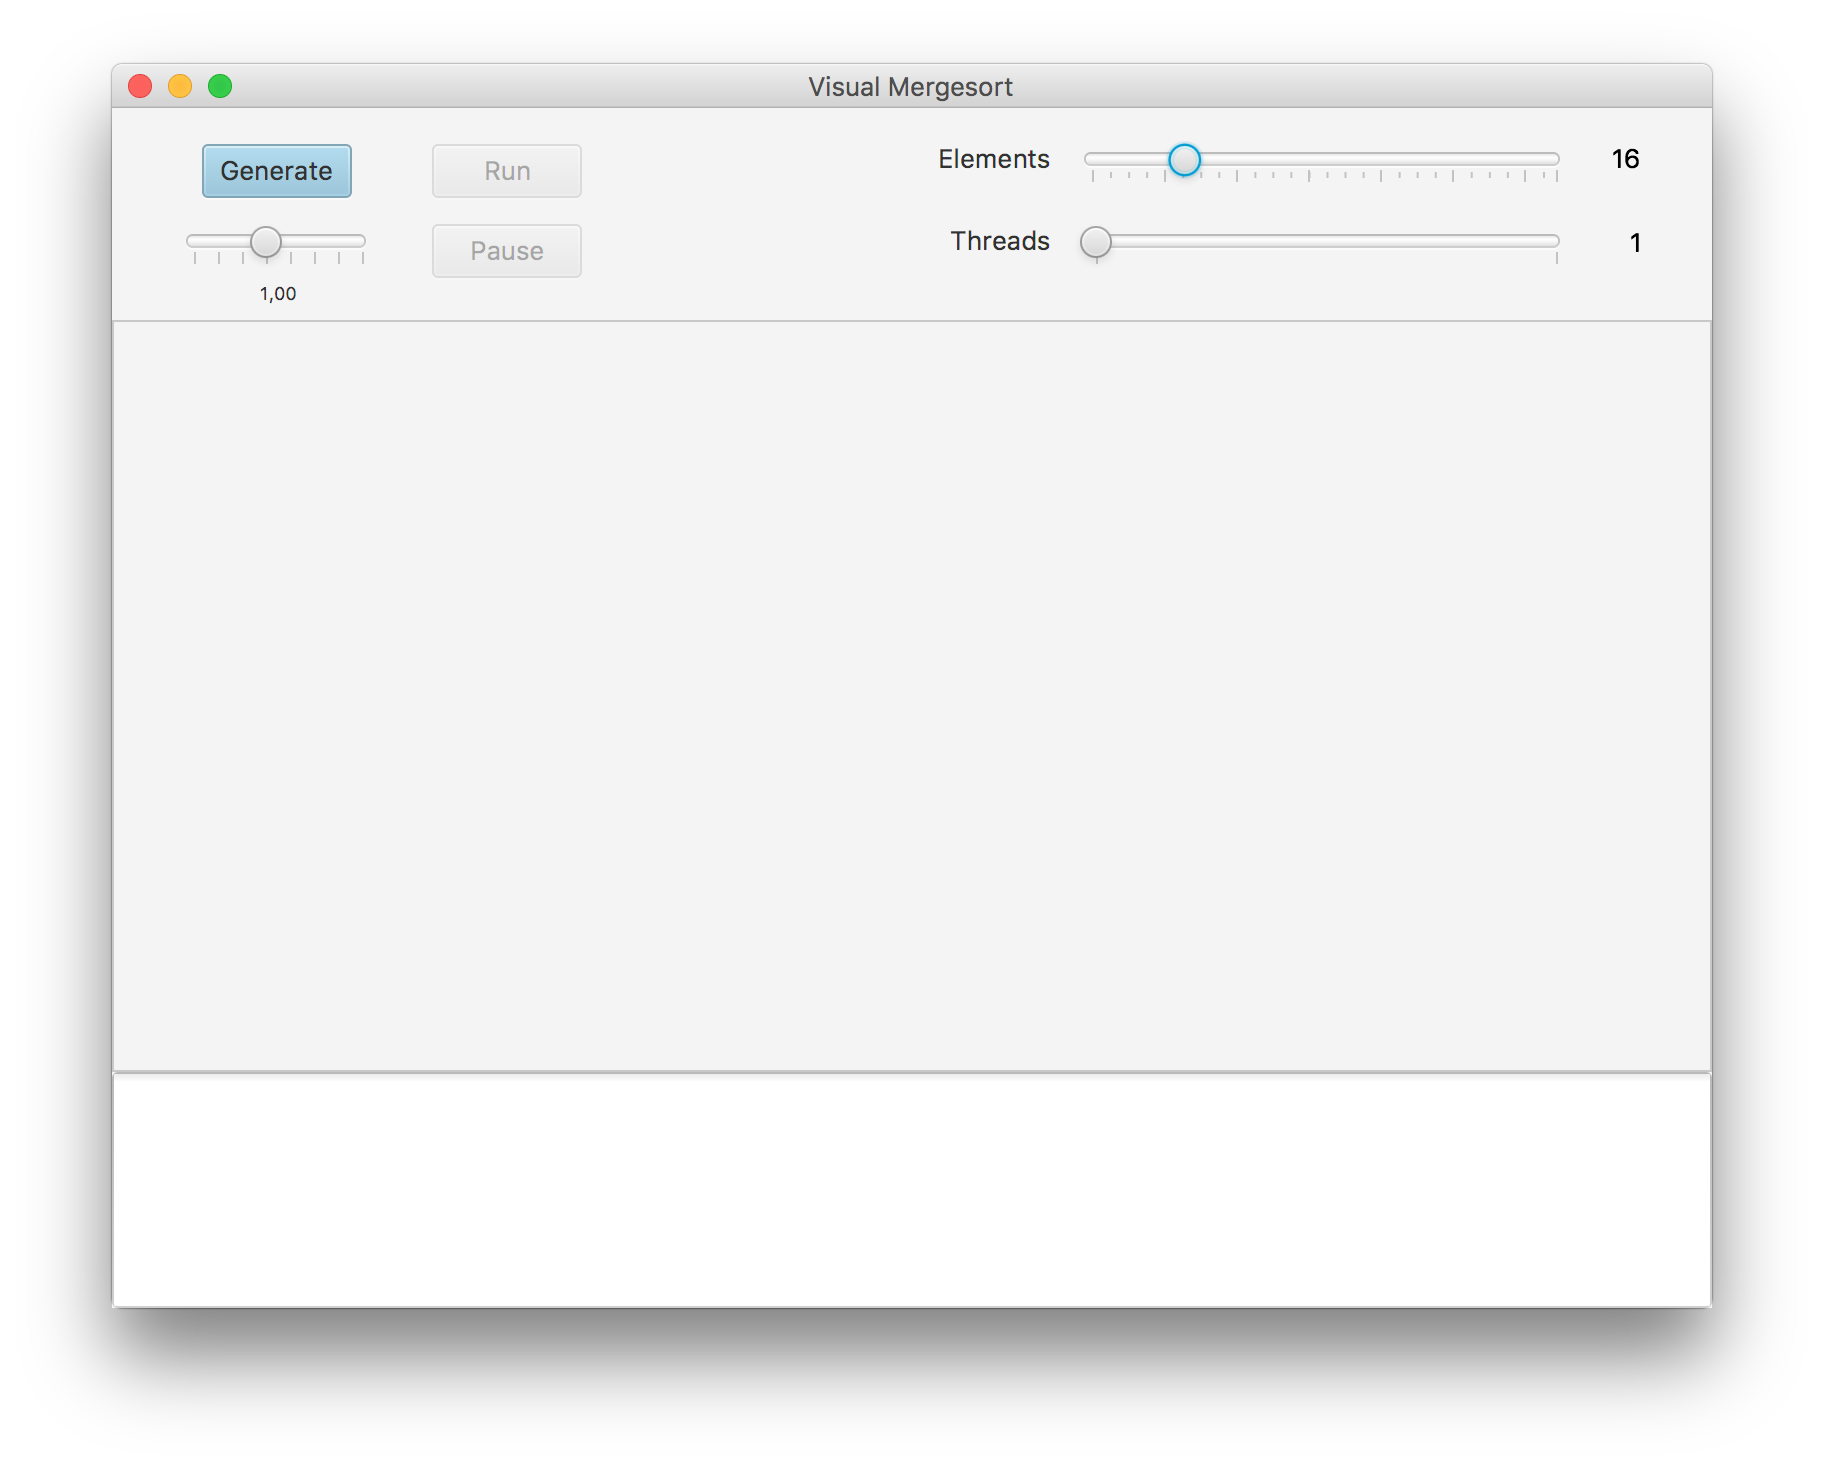
\includegraphics[width=0.75\linewidth]{bild1}
    \caption{Applikation direkt nach dem Starten}
    \label{figure:start-app}
\end{figure}

Über \texttt{ENTER} oder das Klicken auf \texttt{Generate} können direkt die über den Slider voreingestellten 16 Zufallselemente in willkürlicher Reihenfolge generiert werden. Alternativ kann über die Menüleiste \texttt{File} $\rightarrow$ \texttt{Generate Random Data} eine andere Reihenfolge ausgewählt werden. Um einen schnellen Start mit der gewünschten Menge zu ermöglichen, existieren folgende Shortcuts, welche optional verwendet werden können:

Je nach benutztem Shortcut wird eine andere Menge von Elementen auf der Zeichenfläche platziert. Der Slider für die Anzahl der zu zeichnenden Elemente gilt bei allen Optionen, außer bei der generierung von benutzerspezifischen Elementen (siehe unten).

\begin{description}
\item[STRG + B] Generiert eine Menge von Zufallszahlen in willkürlicher Reihenfolge (default).

\begin{figure}[!htb]
    \centering
      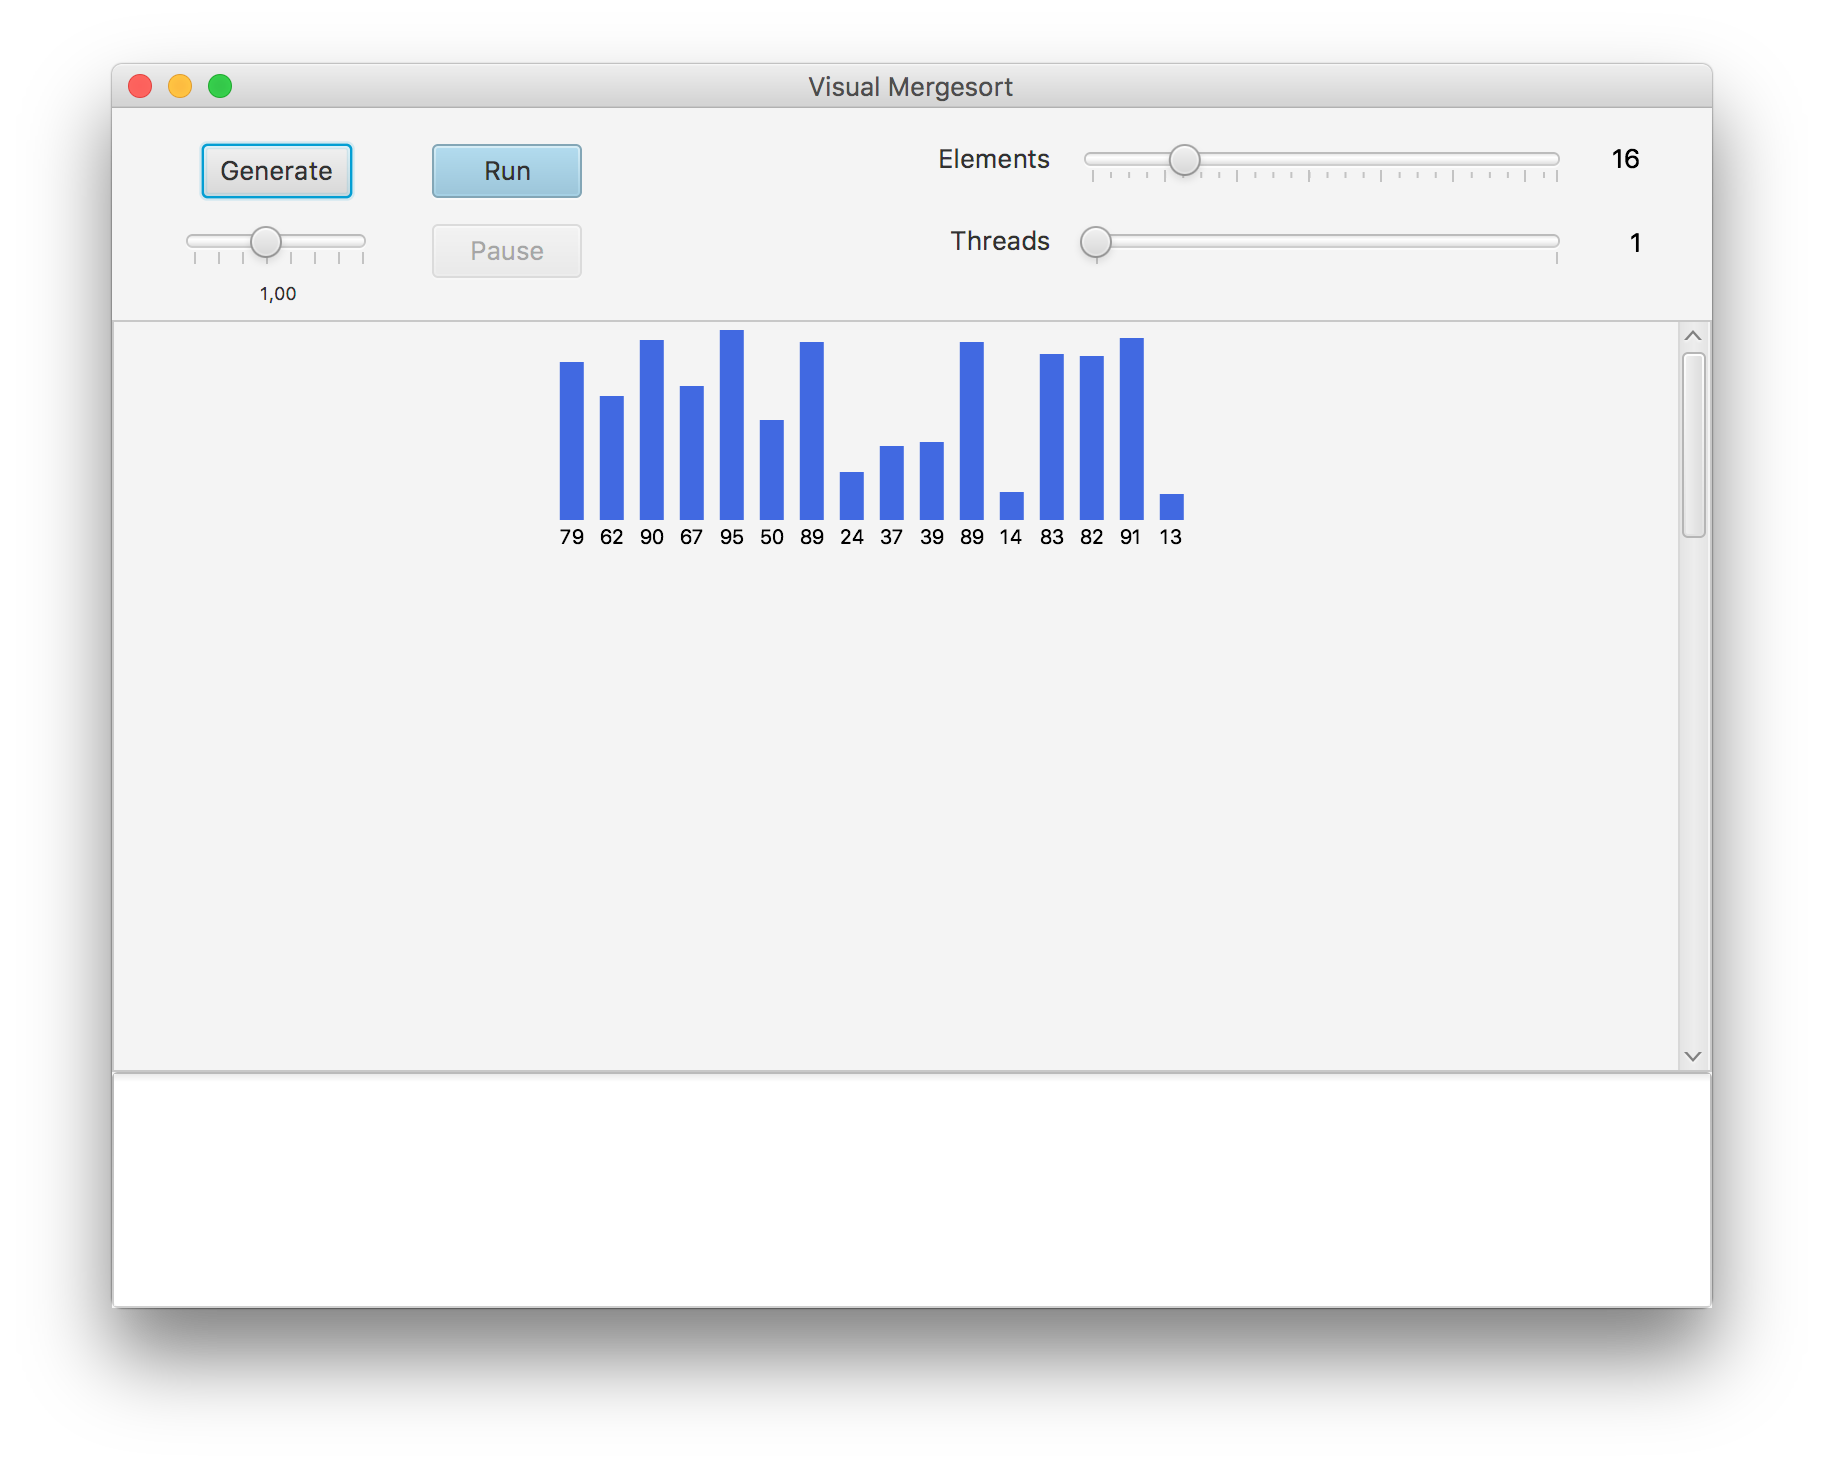
\includegraphics[width=0.75\linewidth]{bild2}
    \caption{Elemente in zufälliger Reihenfolge}
\end{figure}

\item[STRG + O] Generiert eine Menge von Zufallszahlen in vorsortierter, aufsteigender Reihenfolge.

\begin{figure}[!htb]
    \centering
      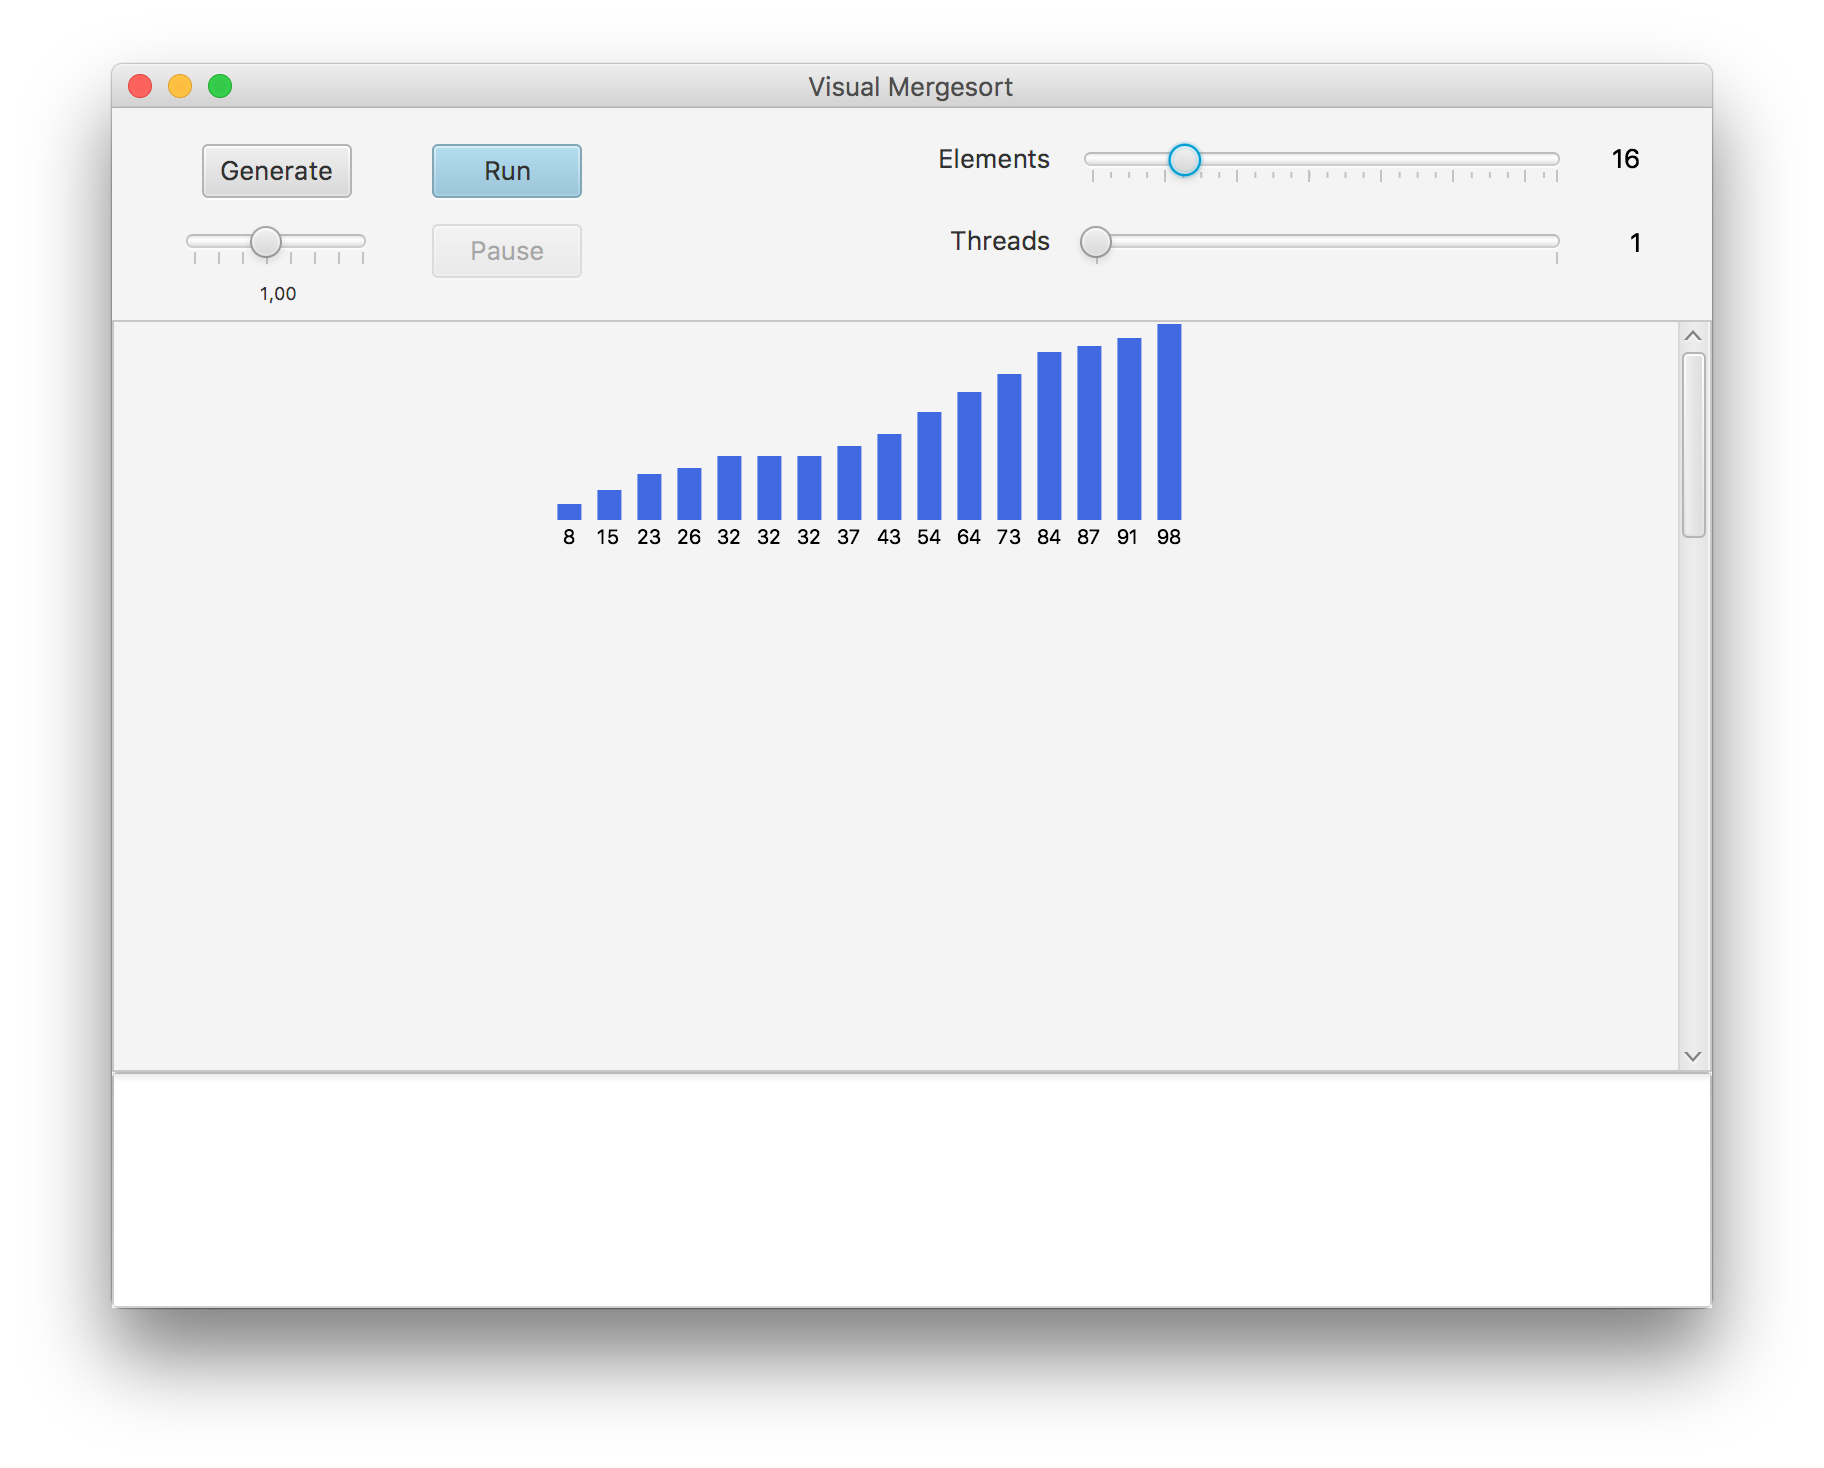
\includegraphics[width=0.75\linewidth]{bild6}
    \caption{Elemente vorsortiert in aufsteigender Reihenfolge}
\end{figure}

\item[STRG + I] Generiert eine Menge von Zufallszahlen, welche absteigend sortiert ist.

\begin{figure}[!htb]
    \centering
      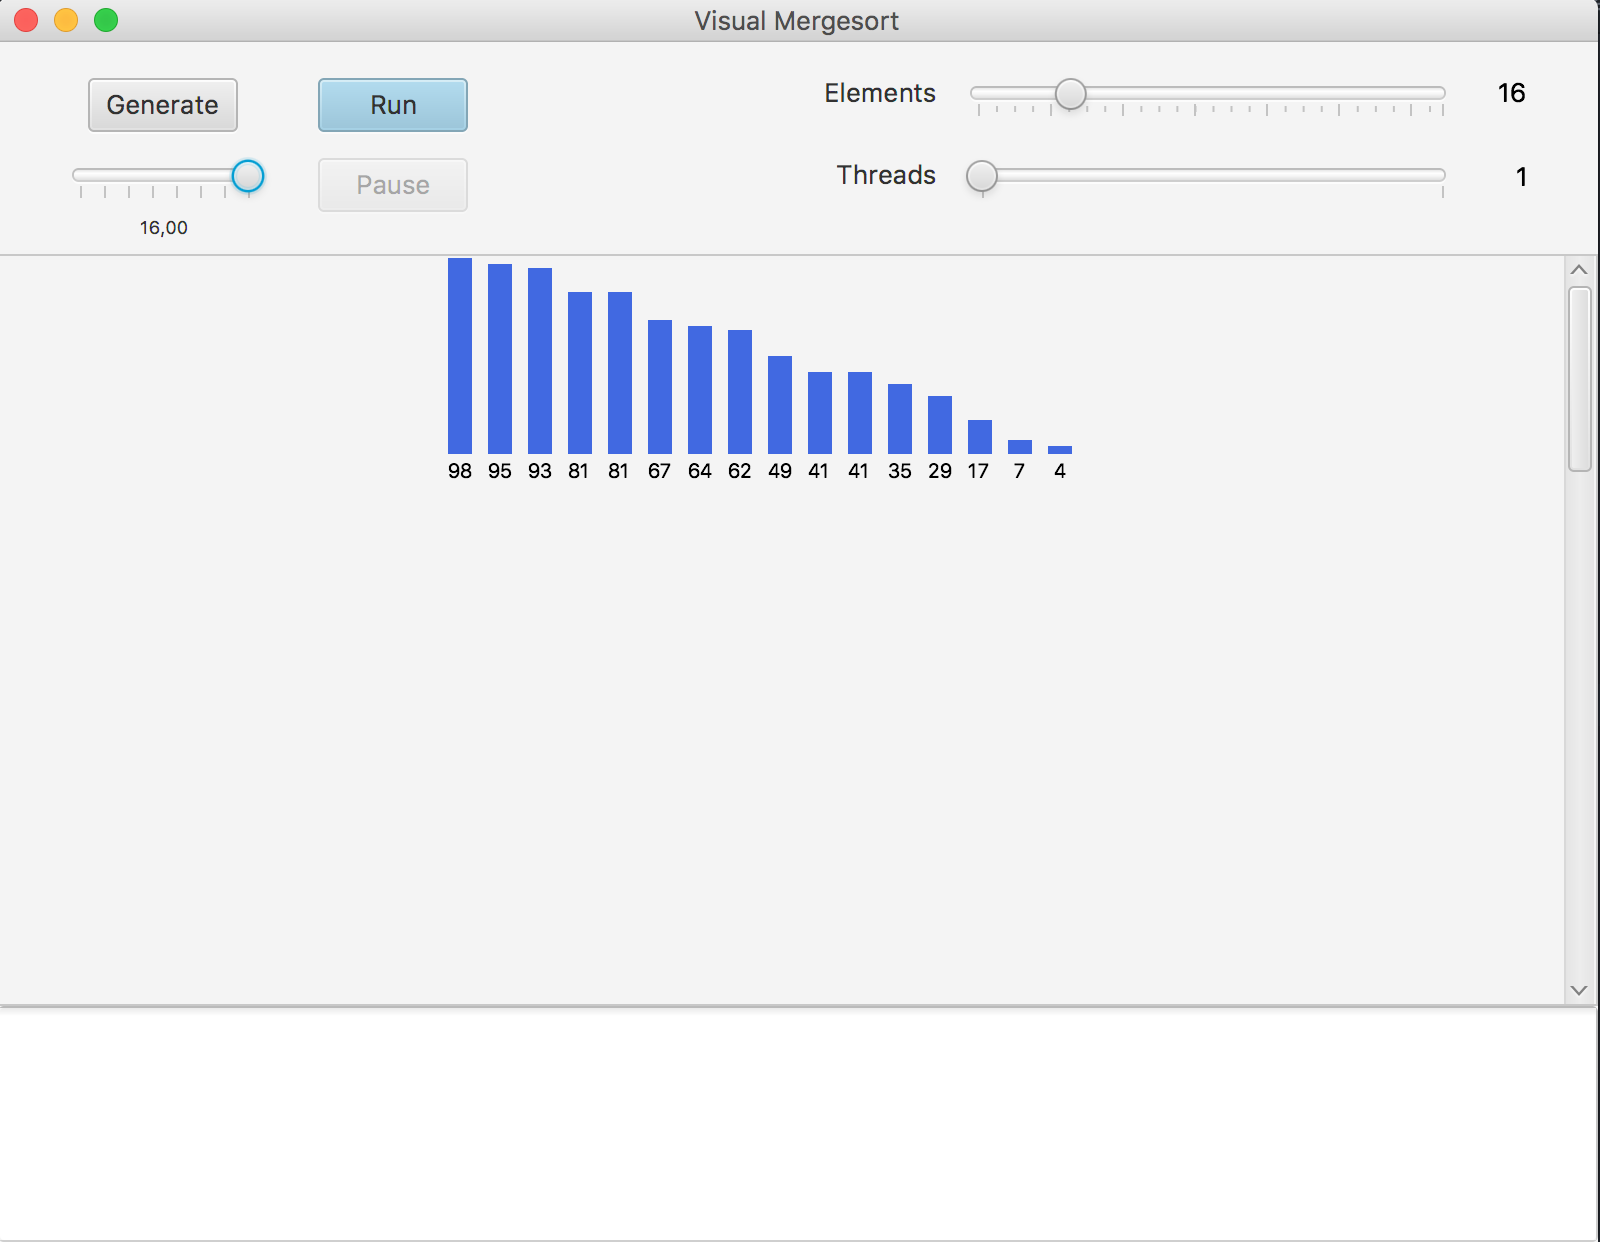
\includegraphics[width=0.75\linewidth]{bild7}
    \caption{Elemente vorsortiert in absteigender Reihenfolge}
\end{figure}

\item[STRG + U] Sowohl die Menge der Zahlen als auch die Reihenfolge kann über den Benutzer manuell eingegeben werden. Hierzu öffnet sich ein Fenster, bei dem die gewünschten Werte eingegeben werden. Dabei ist darauf zu achten, dass jeder Wert durch ein Komma vom nächsten Wert getrennt wird.

\begin{figure}[!htb]
    \centering
      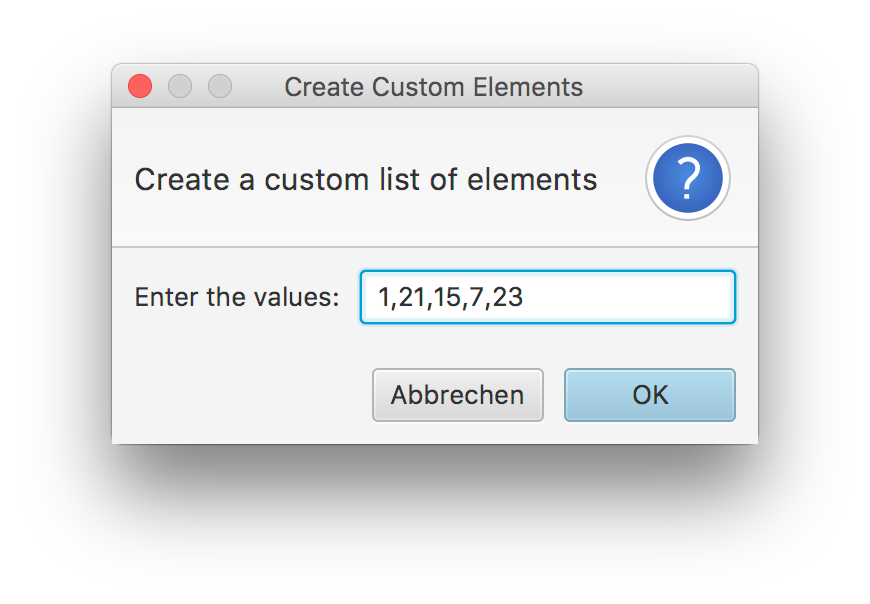
\includegraphics[width=0.75\linewidth]{bild8}
    \caption{Generieren von benutzerspezifischen Elementen}
\end{figure}

Bestätigt man anschließend durch das Drücken auf den Button \texttt{OK}, erscheinen die eingegebenen Werte als Elemente auf der Zeichenfläche

\begin{figure}[!htb]
    \centering
      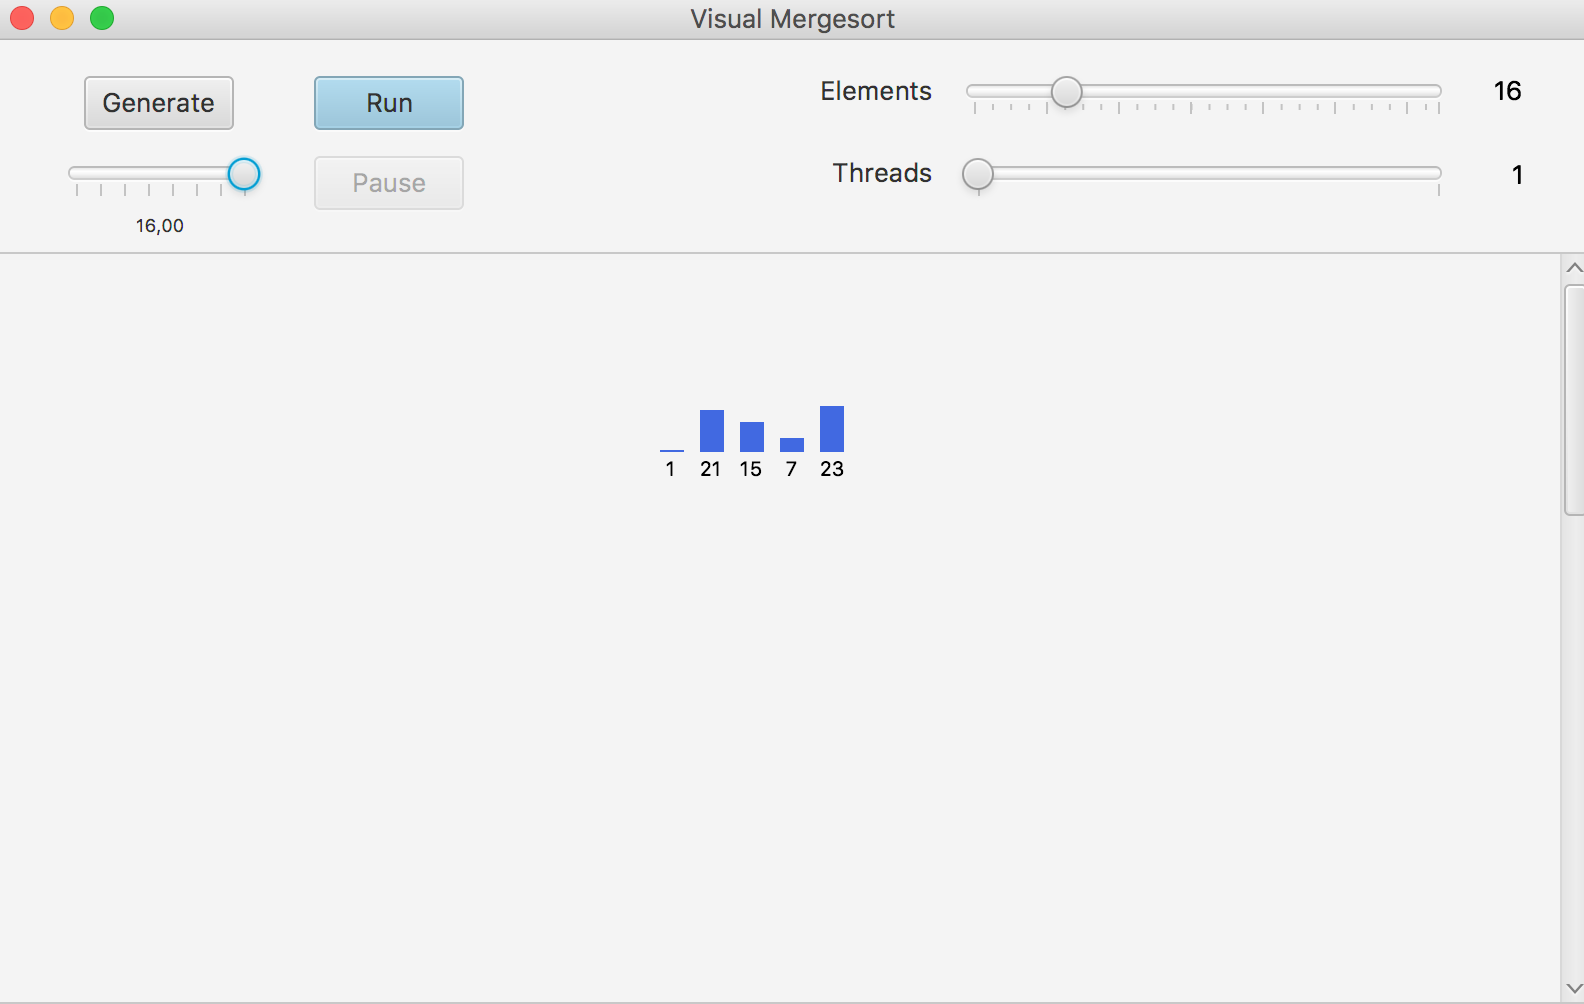
\includegraphics[width=0.75\linewidth]{bild9}
    \caption{Benutzerspezifische Elemente wurden generiert}
\end{figure}
\end{description}





Mit \texttt{ENTER}, einem Klick auf \textbf{Run} oder dem optionalen Shortcut \texttt{STRG + r} wird der Sortieralgorithmus gestartet. Über den Slider mit der Signatur \textit{Threads} kann die Anzahl der für den Algorithmus verwendeten Threads eingestellt werden. Hierbei kann man zwischen einem und zwei Threads wählen.\\
Wurde die Animation gestartet, kann diese jederzeit in ihrer Geschwindigkeit über den Regler unter dem Generate-Button variiert oder über den Button \textit{Pause} bzw. \textit{Play} komplett pausiert bzw. fortgesetzt werden. Beim Starten der Applikation fällt mit Sicherheit auf, dass sich das System automatisch zum Geschehen mitbewegt, um das Vorgehen besser zu visualisieren. Möchte man sich bestimmte Teile genauer ansehen, kann die Anwendung pausiert werden - Anschließend kann man sich frei auf der Zeichenfläche bewegen.

Darüber hinaus kann über den Menüpunkt View die Ansicht der Applikation zu jeder Zeit angepasst werden. Hier existieren die Optionen
\texttt{Toggle Log Console} und \texttt{Toggle Action Bar}. \texttt{Toggle Log Console} sorgt für das Ein- und Ausblenden der Konsole
im unteren Teil der Anwendung. Dadurch kann man bei Bedarf die zusätlichen Informationen zu \texttt{Split} und \texttt{Merge} ausblenden,
um mehr Platz für die eigentliche Animation zu schaffen. \texttt{Toggle Action Bar} ist hierbei aus den gleichen Gründen für das Ein- und Ausblenden
der Schalt- und Kontrollflächen im oberen Teil der Applikation zuständig. Zusätzlich können diese Funktionen optional auch über Tastenkombinationen ausgeführt
werden:

\begin{description}
\item[STRG + K] Blendet die Aktionsbar ein und aus.

\begin{figure}[!htb]
    \centering
      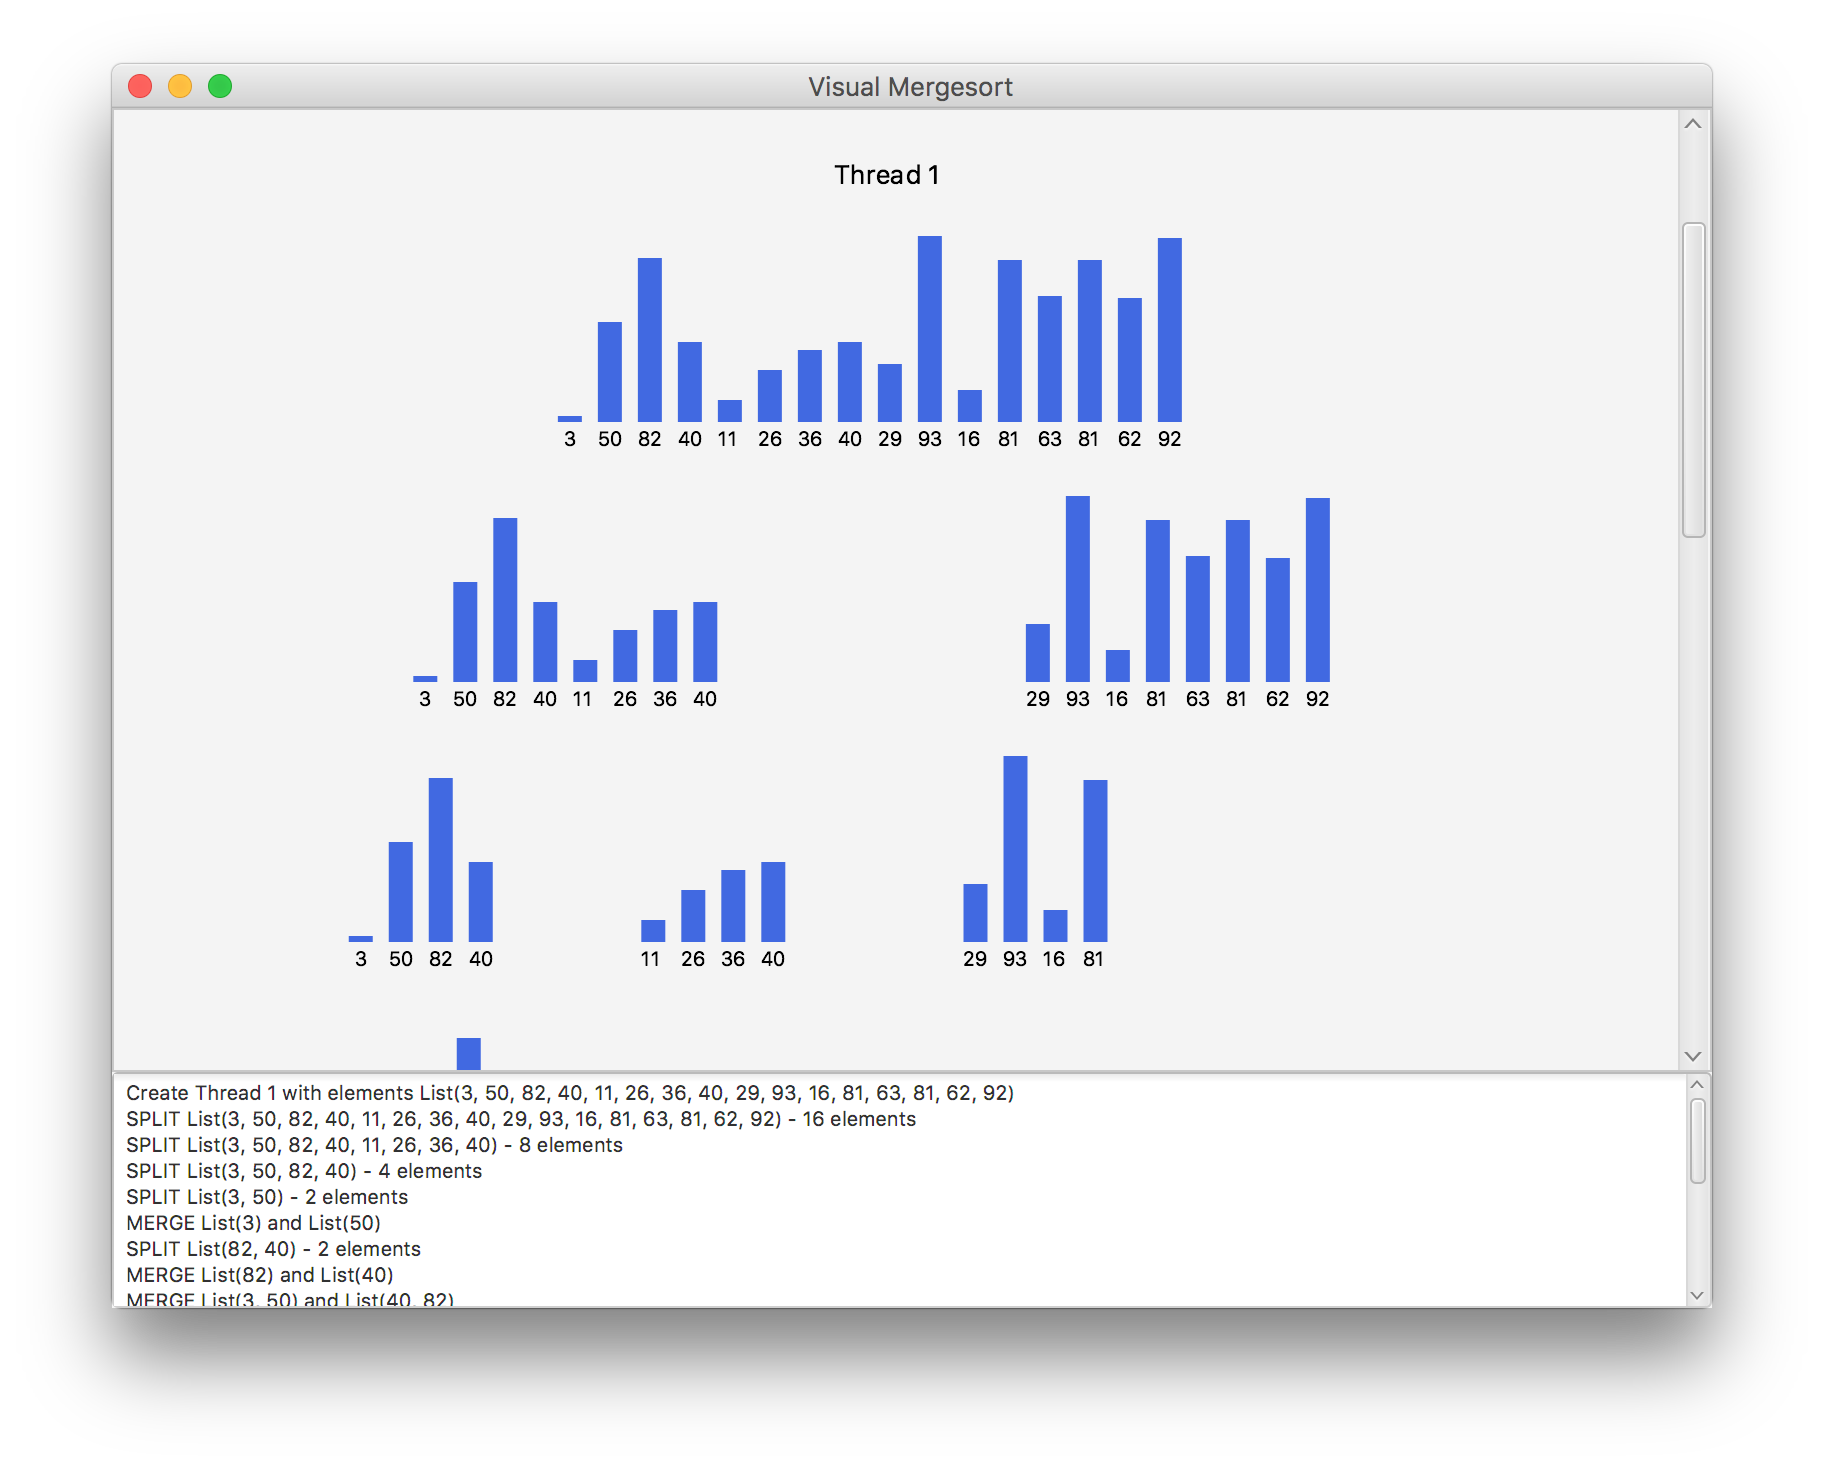
\includegraphics[width=0.85\linewidth]{bild10}
    \caption{Visual Mergesort mit ausgeblendeter Aktionsbar}
\end{figure}

\item[STRG + L] Blendet die Konsole ein und aus.

\begin{figure}[!htb]
    \centering
      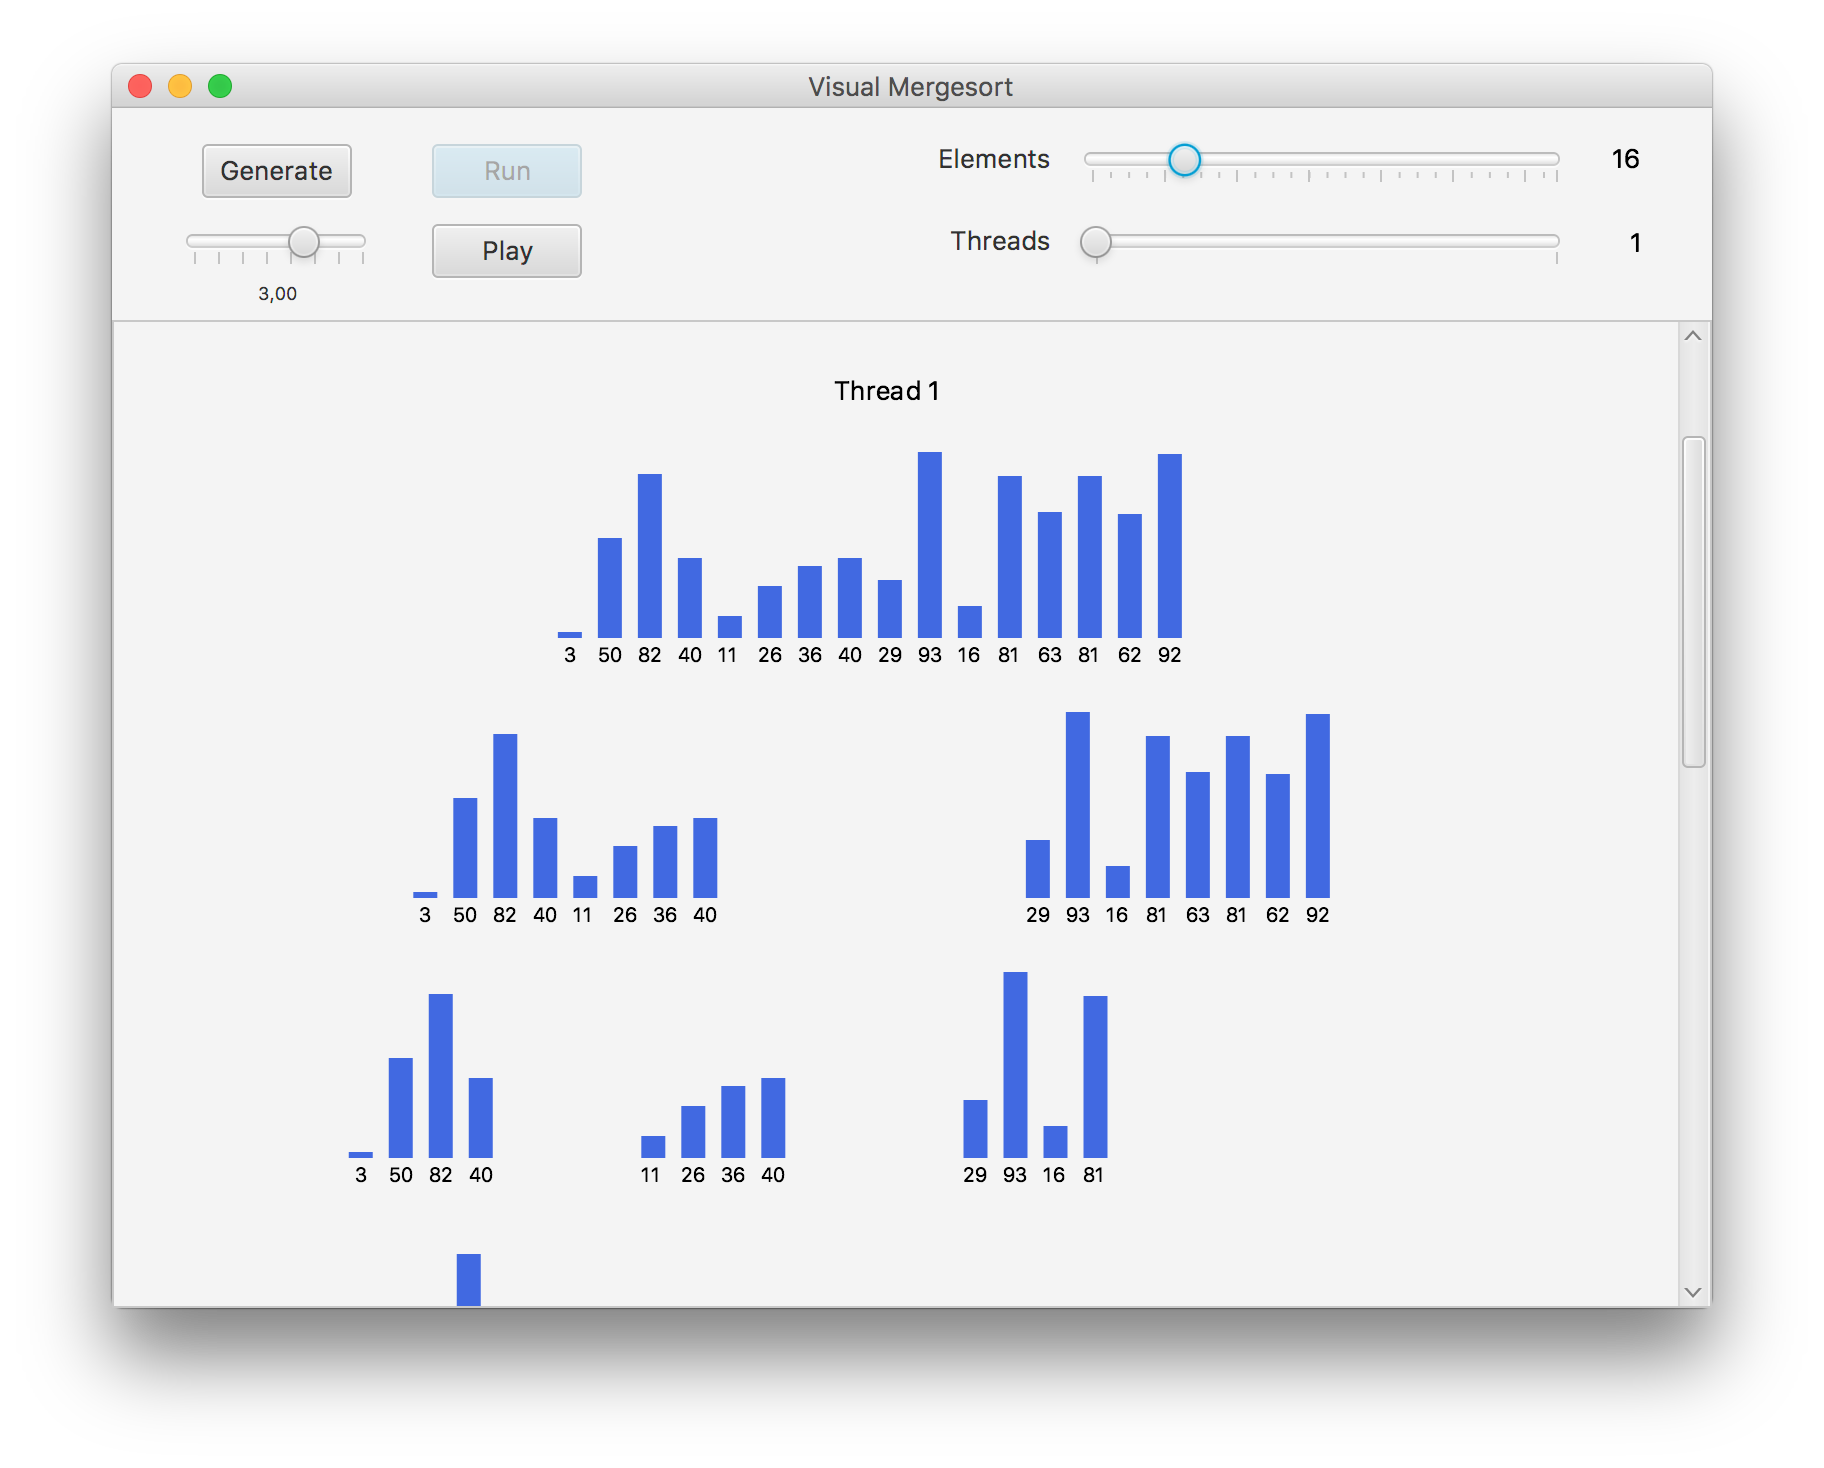
\includegraphics[width=0.75\linewidth]{bild11}
    \caption{Visual Mergesort mit ausgeblendeter Konsole}
\end{figure}
\end{description}

Um den Algorithmus effizienter zu machen, ist es möglich, beim Visual Mergesort die Anzahl der verwendeten Threads, die den Sortieralgorithmus ausführen, zu verändern. Dadurch kann sich der Benutzer vor Augen halten, wie der Mergesort parallelisiert werden kann, um dessen Leistung zu steigern. Wurde über den Slider \texttt{Threads} die Zahl 2 ausgewählt, wird die zu sortierende Liste beim Starten der Anwendung über \texttt{Run} direkt in zwei Listen geteilt, welche jeweils einem \texttt{Thread 1} und einem \texttt{Thread 2} zugewiesen werden:

\begin{figure}[!htb]
    \centering
      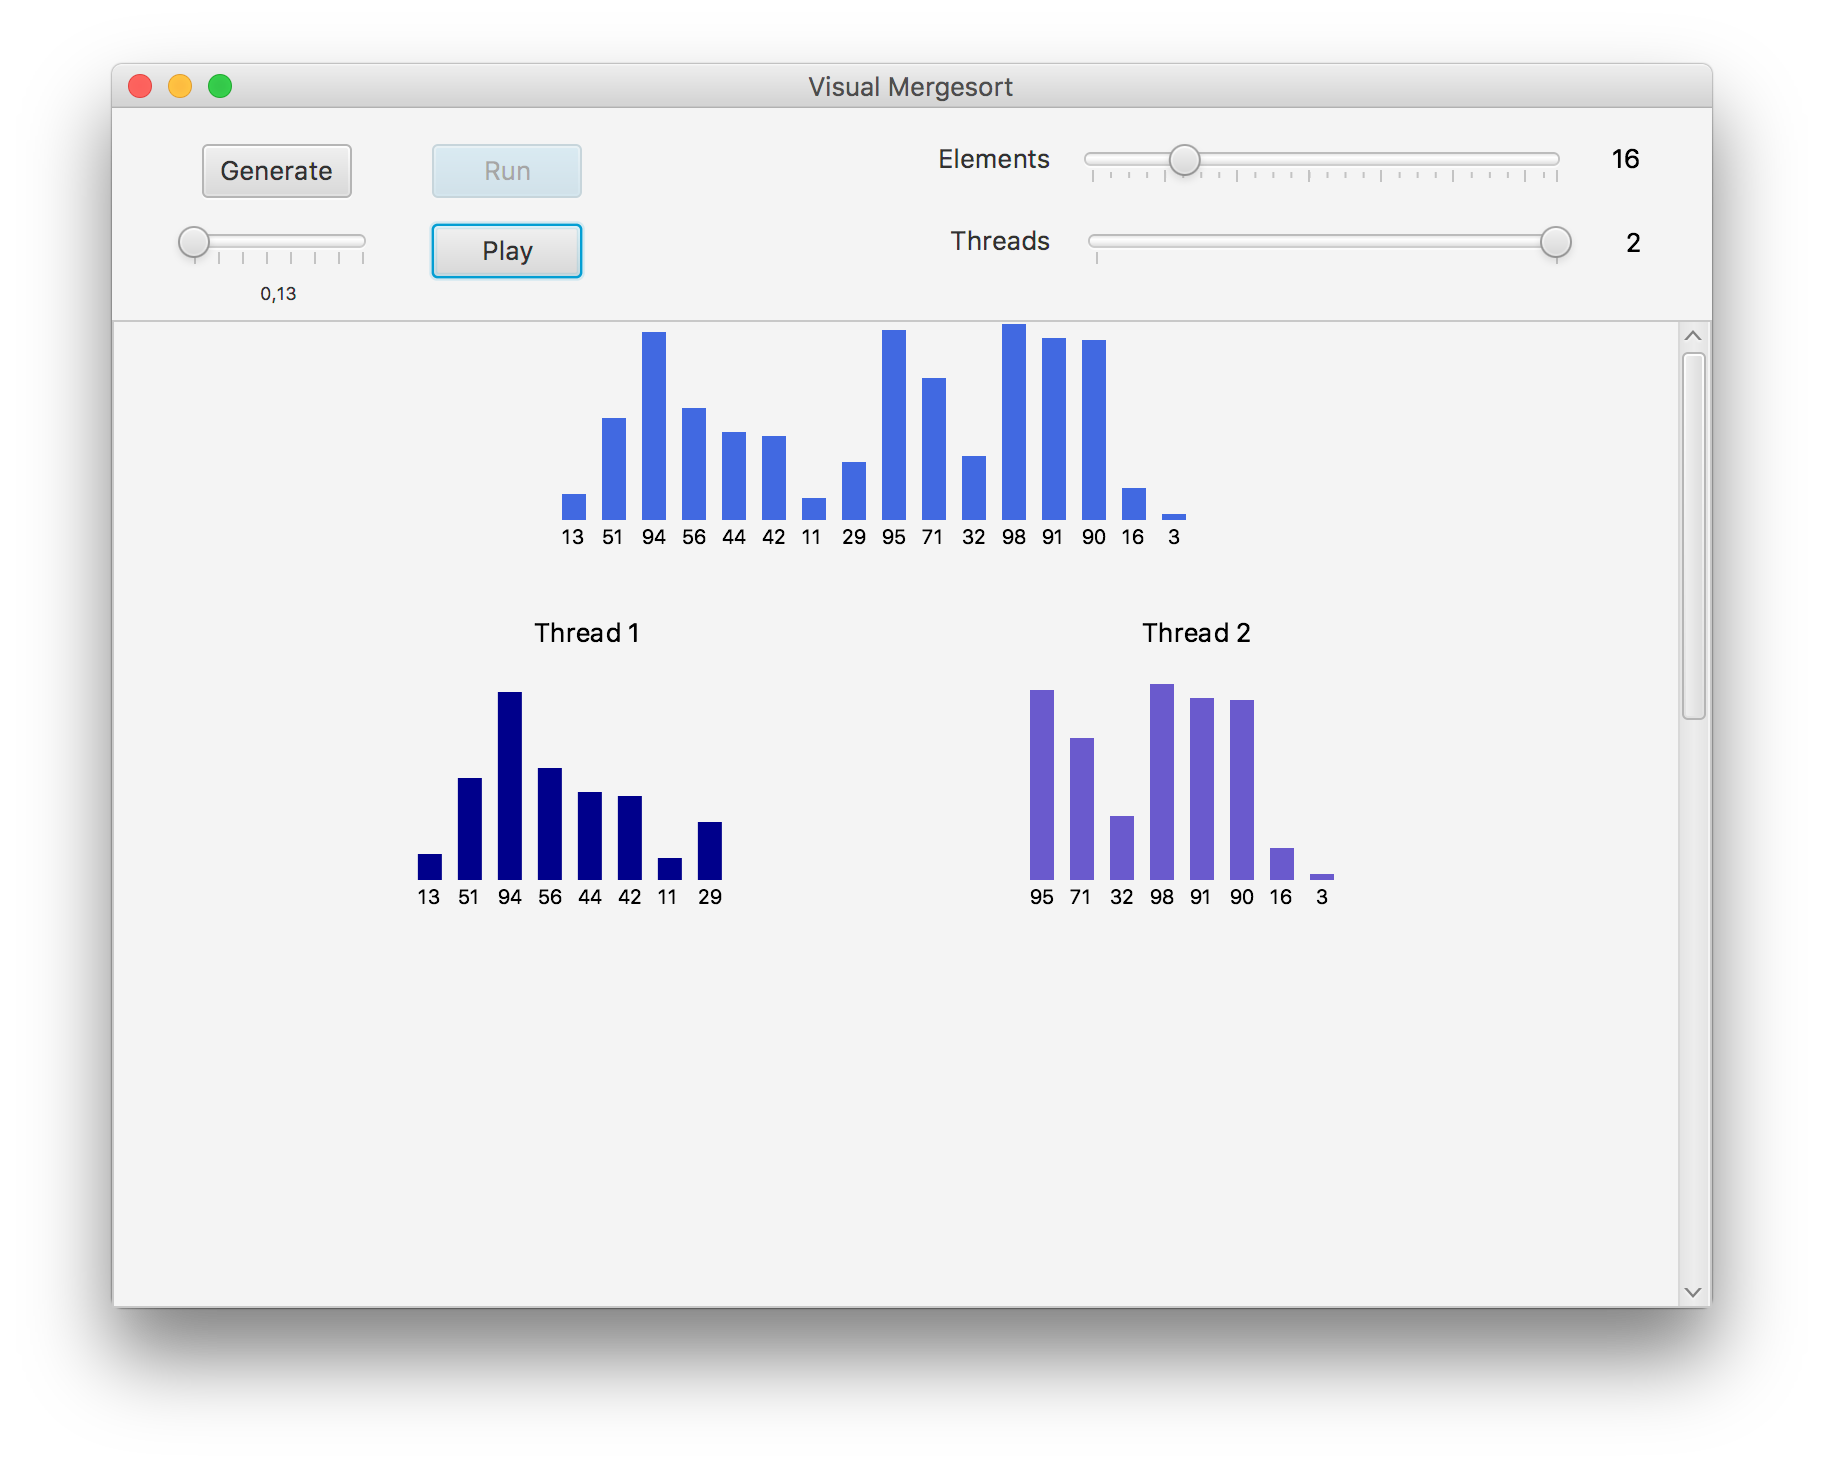
\includegraphics[width=0.75\linewidth]{bild12}
    \caption{Visual Mergesort mit zwei Threads}
\end{figure}

Ab hier führt jeder Thread den Mergesort-Algorithmus für die Liste durch, die ihm zugeteilt wurde, bis diese vollständig sortiert ist. Zum Schluss kommt es zu einem finalen Merge, bei dem die beiden durch die Threads generierten Teillisten zu einer Ganzen zusammengefügt werden. Hierbei kann es, beispielsweise bei einer ungeraden Anzahl an Ausgangselementen dazu kommen, dass ein Thread mehr Zeit benötigt, als der andere, da dieser ein Element weniger sortieren muss. Für diesen Sonderfall wird die Autoscrollfunktion automatisch deaktiviert, da die Threads an verschiedenen Stellen auf der Zeichenfläche arbeiten. Vor dem final Merge wartet der eine Thread auf den anderen, bis dessen Liste auch sortiert ist.

\begin{figure}[!htb]
    \centering
      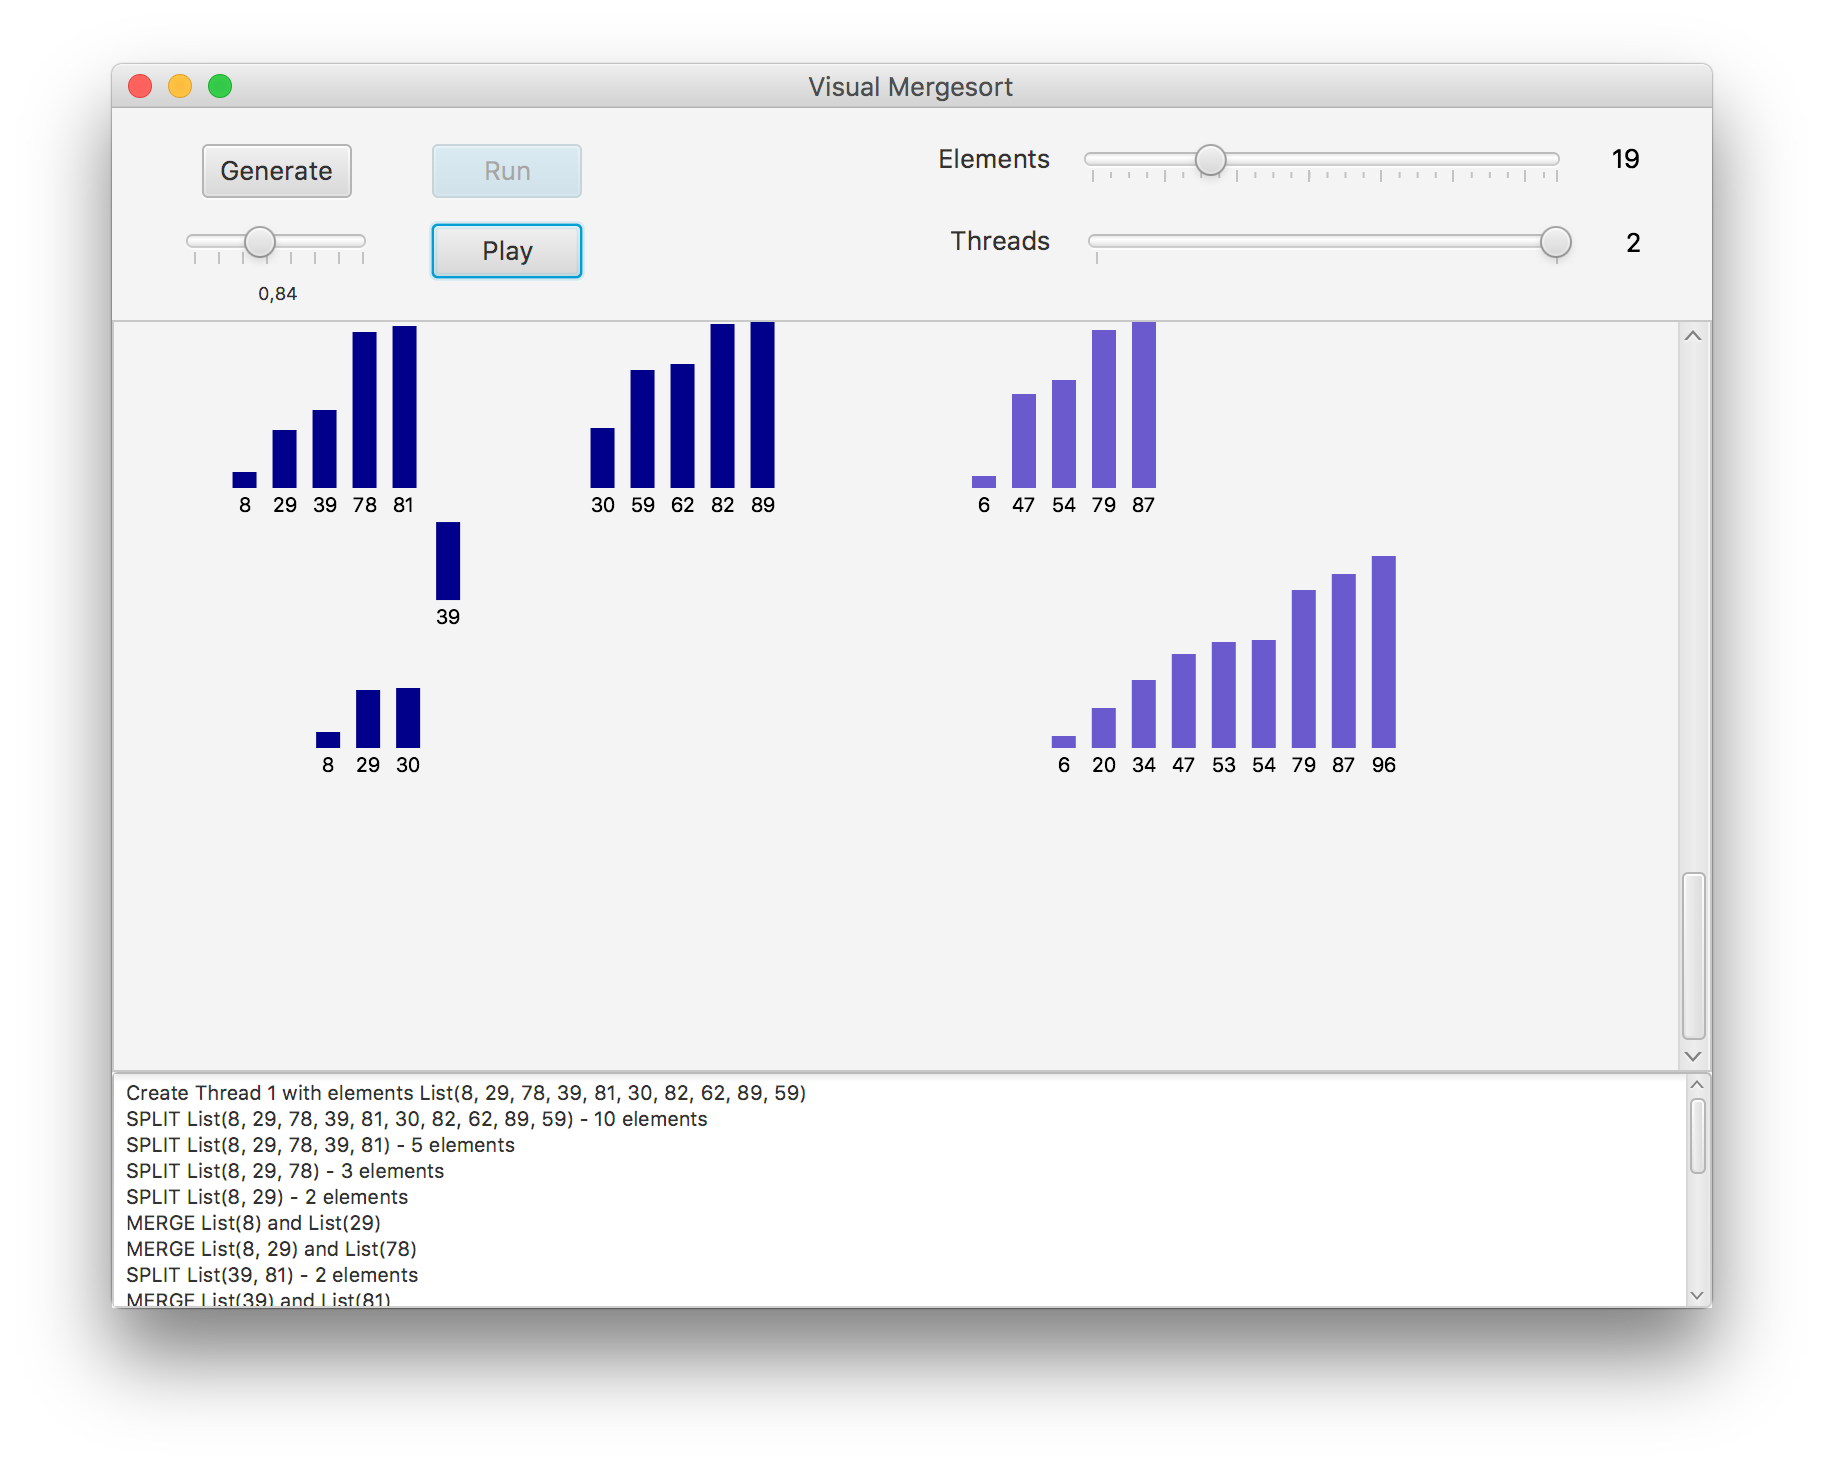
\includegraphics[width=0.75\linewidth]{bild13}
    \caption{Thread 2 wartet auf Thread 1}
\end{figure}

\clearpage
\section{Weiterentwickeln}

Falls man das Programm manuell kompilieren möchte, oder man die Funktionen weiterentwickeln möchte, haben wir hier eine kleine Anleitung: Welche Programme man benötigt, wo welche Dateien liegen, wie man das Programm manuell kompiliert und wie man schlussendlich eine ausführbare Datei bekommt.

\subsection{Voraussetzungen}

Wenn man das Programm selber kompilieren und weiter-entwickeln möchte, benötigt man die folgenden Dinge:

\begin{enumerate}
\item SBT (Scala Build Tool)
\item git
\item JVM und JDK
\end{enumerate}

Wir gehen davon aus, dass sowohl JVM als auch JDK installiert sind. Alternativ kann man auf der Oracle--Seite\footnote{ \url{https://docs.oracle.com/javase/8/docs/technotes/guides/install/install_overview.html}} nachlesen, wie man diese für sein Betriebssystem installiert.

Das Scala Built Tool kann man auf der Projektseite\footnote{\url{http://www.scala-sbt.org/index.html}} herunter laden, und im Anschluss kann man dieses installieren. Über dieses Build Tool wird dann später Scala in der entsprechenden Version geladen, sodass man Scala selber nicht installieren muss. Möchte man Scala dennoch installieren, um beispielsweise die \texttt{REPL} \cite{GettingStartedWithTheScalaREPL} zu nutzen, so kann man Scala über die Webseite\footnote{\url{http://scala-lang.org/}} herunter laden.

Zuletzt benötigt man noch git\footnote{\url{https://git-scm.com/book/en/v2/Getting-Started-Installing-Git}}, um das Projekt über Github beziehen zu können.

\subsection{Programm starten}

Im Nachfolgenden werden die Befehle aus im Terminal ausgeführt. Diese Schritt-für-Schritt--Anleitung wurde auf Linux und OSX getestet, sollte jedoch auf Windows ähnlich funktionieren.

Zuerst muss das Projekt von Github geladen werden. Über git kann man den folgenden Befehl ausführen, um das Projekt von Github zu \texttt{clonen}.

\begin{verbatim}
git clone https://github.com/TobsCore/Visual-Mergesort.git
\end{verbatim}

Es ist ein neues Verzeichnis mit den Projektdaten erstellt worden. Wenn man in dieses Verzeichnis navigiert, befinden sich dort zwei Ordner und eine \texttt{README.md} Datei.

\begin{verbatim}
cd Visual-Mergesort/
ls
\end{verbatim}

In den Ordnern befinden sich die folgenden Daten:

\begin{description}
\item[Code/] In diesem Ordner ist das eigentliche Programm enthalten, sowie die sbt--Konfiguration und die Intellij Dateien.
\item[Documentation/] Hier ist die Dokumentation über unsere Projektarbeit enthalten, die wir geschrieben habe. Die Dokumentation ist in \LaTeX~ geschrieben und kann über \texttt{xelatex} kompiliert werden. Mehr dazu in \ref{sec:latex}.
\end{description}

Wenn man nun in den \texttt{Code/} Ordner wechselt, befinden sich darin wiederrum 4 Ordner (3 sichtbar, 1 nicht sichtbar):

\begin{description}
\item[project/] Hier sind die sbt Projektdateien enthalten.
\item[src/] Dies ist der wichtigste Unterordner. Hier ist der Programmcode enthalten, da es sich um den \texttt{Source}--Ordner handelt.
\item[target/] Hier landen kompilierte Dateien und Caches. Die ausführbare \texttt{Visual-Mergesort"".jar}--Datei wird beispielsweise auch in diesen Ordner geschrieben.
\item[.idea/] Dies ist der Intellij Projektordner.
\end{description}

Zuletzt möchten wir noch die Ordnerstruktur des \texttt{src/} Ordners erklären. In dem Unterordner \texttt{main/} befinden sich noch die Ordner \texttt{resources/} und \texttt{scala/}. In \texttt{resources/}, sind Bilder, die CSS Dateien und die \texttt{FXML} Dateien enthalten. Der ganze Programmcode ist in dem Ordner \texttt{scala/}.

Um das Programm nun kompilieren zu können, gehen wir zurück in den Ordner \texttt{Visual-Mergesort""/Code/}. In diesem Ordner sollte sich eine Datei mit dem Namen \texttt{build.sbt} befinden. Wenn man nun den Befehl

\begin{verbatim}
sbt compile
\end{verbatim}

ausführt, so wird der Programmcode kompiliert und kann im Anschluss über

\begin{verbatim}
sbt run
\end{verbatim}

ausgeführt werden. Nun wird die Anwendung gestartet.

\subsubsection{Ausführbare Datei erstellen}
Da man nicht immer den Programmcode beziehen und kompilieren möchte, ist es sinnvoll, wenn man sich eine ausführbare Anwendung erstellen lässt. Dies ist, wie bereits erwähnt, eine Datei mit der Endung \texttt{.jar}. Wir benutzen ein sbt--Plugin, das sich um die Erstellung dieser Datei kümmert. Man kann die Erstellung über

\begin{verbatim}
sbt assembly
\end{verbatim}

anstoßen. Die generierte Datei liegt dann in dem Ordner \texttt{target/scala-2.11/} und heißt \texttt{Visual-Mergesort.jar}. Mit

\begin{verbatim}
java -jar Visual-Mergesort.jar
\end{verbatim}

kann man die Anwendung starten.

\subsection{Dokumentation}\label{sec:latex}

Die Dokumentation ist in \LaTeX ~geschrieben und kann über \texttt{xelatex} erstellt werden. Das Programm kann auf Linux, Windows und OSX installiert werden. Wir haben zusätzlich ein \texttt{Makefile} angelegt, das das Kompilieren und anschließende Aufräumen für uns übernimmt. Zusätzlich kann man hierüber auch die \texttt{Bibtex} Datei in das Dokument einbauen. \texttt{BibTex} wird genutzt, um die Literaturquellen zu verwalten. Die Datei \texttt{Documentation/README.md}\footnote{Auch hier zu finden: \url{https://github.com/TobsCore/Visual-Mergesort/blob/master/Documentation/README.md}} beschreibt, welche Befehle man über Make\footnote{Es kann sein, dass man das Make--Progamm installieren muss, um das Makefile nutzen zu können. Dies war bei uns zumindest auf Windows--Systemen der Fall} ausführen kann und was diese Befehle bewirken.
